\documentclass[12pt]{article}
\usepackage[a4paper,margin=1in]{geometry}
\usepackage[T1]{fontenc}
\usepackage[utf8]{inputenc}
\usepackage{graphicx}
\usepackage{booktabs}
\usepackage{multirow}
\usepackage{array}
\usepackage{setspace}
\usepackage{float}
\usepackage{amsmath}
\usepackage{xcolor}

\title{\textbf{Mirror Reflection Agent: A Structured Reliability-Control Architecture with Science-Facing Mechanism Evidence for Bounded Scientific Reasoning}}
\author{Brook \\ Independent Researcher}
\date{}

\begin{document}
\maketitle
\onehalfspacing
\emergencystretch=2em

\begin{abstract}
Large language models are increasingly used in scientific workflows, yet their practical usefulness is still constrained by unsupported certainty, failure to preserve source conditions, and weak retention of prior corrections. We present Mirror Reflection Agent, a structured reliability-control architecture that externalizes candidate cognition as a \texttt{MindState}, critiques it through typed \texttt{MirrorVerdict} decisions, and stores correction lineage and reusable strategy traces in memory. The contribution is not a claim of broad AI-for-Science superiority. The contribution is an auditable systems mechanism for improving bounded scientific reasoning behavior. We evaluate the current implementation with a deterministic three-track benchmark that avoids LLM-as-judge scoring. The benchmark contains 98 cases and 354 executed runs across a five-way ablation track, a science-facing question-answering track, and a longitudinal correction-retention track. In Track A, pass rate rises from 0.20 in the direct-answer and structured-cognition baselines to 0.80 in the dual-memory configuration, while correction retention rises from 0.00 to 0.67 and unsupported certainty falls from 0.47 to 0.17. In Track B, reflective modes preserve evidence citation and abstention behavior much better than a naive direct baseline, although condition-sensitive property cases still reveal a coverage--calibration tradeoff. In Track C, cross-session correction retention reaches 0.80 in reflective memory modes versus 0.00 for the direct baseline, with zero measured shared-memory pollution risk. We therefore position the present work as a science-facing systems and mechanism study: the architecture demonstrates bounded reliability gains, but it does not yet establish broad scientific superiority.
\end{abstract}

\noindent\textbf{Keywords:} reflective agents, reliability control, bounded scientific reasoning, memory, uncertainty, AI for science

\section{Introduction}

Scientific uses of language models require more than fluent text generation. A useful system must preserve source conditions, distinguish strong evidence from weak prior knowledge, avoid overclaiming when data are missing, and remember prior corrections without blindly replaying stale templates. Existing reflective pipelines improve outputs through refinement, retrieval, or tool use, but three reliability gaps remain common. First, intermediate reasoning is often not represented as an inspectable state object. Second, critique outcomes are rarely encoded as explicit control decisions that determine whether the system should revise, retrieve, defer, diverge, or pass. Third, prior corrections are often stored as unstructured text rather than as reusable correction lineage.

Mirror Reflection Agent addresses those gaps with an explicit reliability-control architecture. The system builds a structured \texttt{MindState}, critiques it with a mirror layer that emits typed \texttt{MirrorVerdict} actions, and then either revises, retrieves memory, diverges to a new scaffold, waits, or finalizes. Memory stores facts, contexts, bias lineage, correction lineage, and reusable strategy signals. The system is engineering-oriented. It does not claim subjective awareness, consciousness, or human-like introspection. Its aim is narrower: improve auditable, bounded scientific reasoning behavior through explicit state, typed critique, and correction-lineage memory.

The present manuscript makes three bounded contributions. First, it defines a reliability-control architecture centered on explicit candidate state and explicit verdict-typed control flow. Second, it contributes a deterministic three-track evaluation protocol aligned to the strongest criticism of earlier drafts: the previous benchmark was too small, too weakly ablated, and too weakly tied to science-facing tasks. Third, it reports mechanism evidence from a 98-case, 354-run benchmark rather than from a minimal four-case pilot alone.

We organize the paper around three research questions:
\begin{itemize}
\item \textbf{RQ1.} What is the net contribution of each control-flow component when the same tasks are executed under direct-answer, structured-cognition, mirror, local-memory, and dual-memory configurations?
\item \textbf{RQ2.} Does the architecture improve reliability on scientific questions that require numeric correctness, condition preservation, evidence citation, or abstention under insufficient evidence?
\item \textbf{RQ3.} Can correction lineage be retained across sessions without contaminating project-local behavior or producing unsafe shared-memory artifacts?
\end{itemize}

The paper is strongest as a systems and mechanism study with science-facing evidence, rather than as a full scientific-benchmark paper. That boundary is explicit throughout the manuscript: some components are implemented in code, some are exercised in the present benchmark, and broader scientific coverage remains future work.

\section{Results}

\subsection{R1. Architecture claim and validated scope}

Mirror Reflection Agent follows the control flow
\begin{center}
\texttt{input $\rightarrow$ knowledge layers $\rightarrow$ cognition $\rightarrow$ mirror critique $\rightarrow$ revise/retrieve/diverge/wait/pass $\rightarrow$ output $\rightarrow$ memory write-back}
\end{center}
and treats reliability as a control problem rather than as a prompt-only stylistic refinement problem.

\begin{figure}[H]
\centering
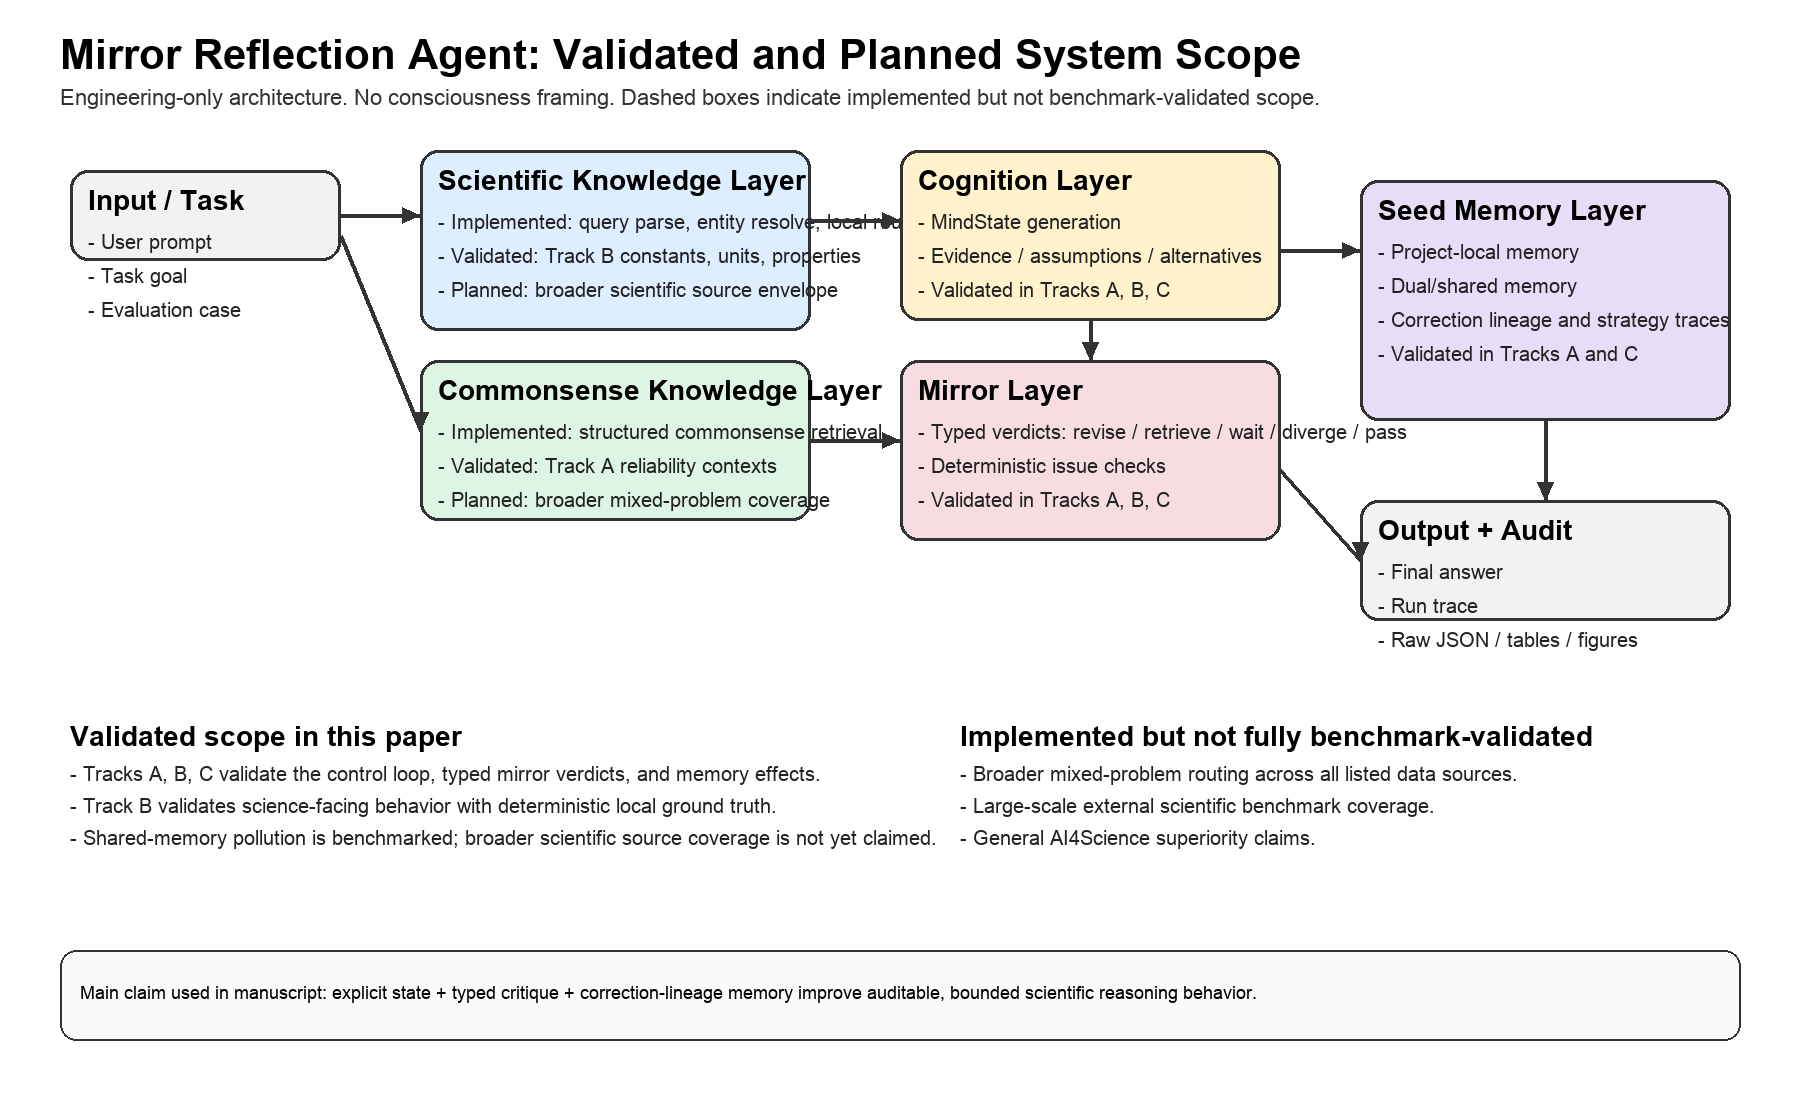
\includegraphics[width=\textwidth]{figure1_architecture_v5.png}
\caption{Figure 1. Engineering schematic of Mirror Reflection Agent with validated and planned scope separated explicitly. The figure uses only implementation-level labels and distinguishes benchmark-validated components from broader planned scientific coverage.}
\label{fig:v5-architecture}
\end{figure}

Figure~\ref{fig:v5-architecture} makes the manuscript's scope boundary explicit. The validated claim in this paper is not that the entire system envelope has been exhaustively benchmarked. The validated claim is that explicit state externalization, typed mirror verdicts, and correction-lineage memory improve reliability-oriented behavior in the current benchmark. Broader mixed-problem routing and large-scale scientific source coverage remain implemented only partially or remain planned.

\begin{table}[H]
\centering
\resizebox{\textwidth}{!}{%
\begin{tabular}{lccccc}
\toprule
Method family & Externalized state & Typed verdicts & Correction lineage & Abstention governance & Science-facing condition handling \\
\midrule
Self-Refine & limited & no & no & no & limited \\
Reflexion & partial & no & partial & limited & no \\
CRITIC & partial & no & no & limited & tool-dependent \\
Self-RAG & partial & partial & no & limited & retrieval-aware only \\
Mirror Reflection Agent & explicit & yes & yes & yes & yes, within current local data envelope \\
\bottomrule
\end{tabular}
}
\caption{Table 1. Novelty-isolation table. The intended contribution of the present work is the combined use of explicit state externalization, typed control verdicts, persistent correction lineage, abstention governance, and science-facing condition handling.}
\label{tab:v5-novelty}
\end{table}

Table~\ref{tab:v5-novelty} isolates the intended novelty relative to closely related reflective pipelines. The main difference is not simply "more reflection." It is the combination of explicit state objects, typed control actions, persistent correction-lineage memory, and science-facing evidence constraints within a single inspectable control loop.

\subsection{R2. Track A: complete ablation answers the baseline problem}

Track A directly answers reviewer 2's strongest criticism of the earlier manuscript: the prior comparison did not isolate where the gains came from. The new ablation contains 30 cases spanning six reliability families and five thematic variants. Each case is executed under five configurations:
\begin{enumerate}
\item \texttt{direct\_answer}
\item \texttt{mindstate\_only}
\item \texttt{mindstate\_mirror}
\item \texttt{mindstate\_mirror\_local\_memory}
\item \texttt{mindstate\_mirror\_dual\_memory}
\end{enumerate}

\begin{table}[H]
\centering
\resizebox{\textwidth}{!}{%
\begin{tabular}{lcccccccc}
\toprule
Mode & Cases & Pass & Rev. succ. & Premature conv. & Concept mix & Corr. retain & Unsup. cert. & Avg. conf. \\
\midrule
Direct answer & 30 & 0.20 & 0.00 & 0.00 & 0.00 & 0.00 & 0.47 & 0.88 \\
MindState only & 30 & 0.20 & 0.00 & 0.17 & 0.00 & 0.00 & 0.47 & 0.68 \\
MindState + Mirror & 30 & 0.33 & 0.17 & 0.17 & 0.00 & 0.00 & 0.33 & 0.50 \\
Mirror + local memory & 30 & 0.63 & 0.17 & 0.17 & 0.03 & 0.33 & 0.33 & 0.54 \\
Mirror + dual memory & 30 & 0.80 & 0.33 & 0.00 & 0.20 & 0.67 & 0.17 & 0.52 \\
\bottomrule
\end{tabular}
}
\caption{Table 2. Track A five-way ablation aggregate over 30 cases. ``Rev. succ.'' denotes revision success rate; ``Unsup. cert.'' denotes unsupported-certainty rate.}
\label{tab:v5-track-a-aggregate}
\end{table}

\begin{figure}[H]
\centering
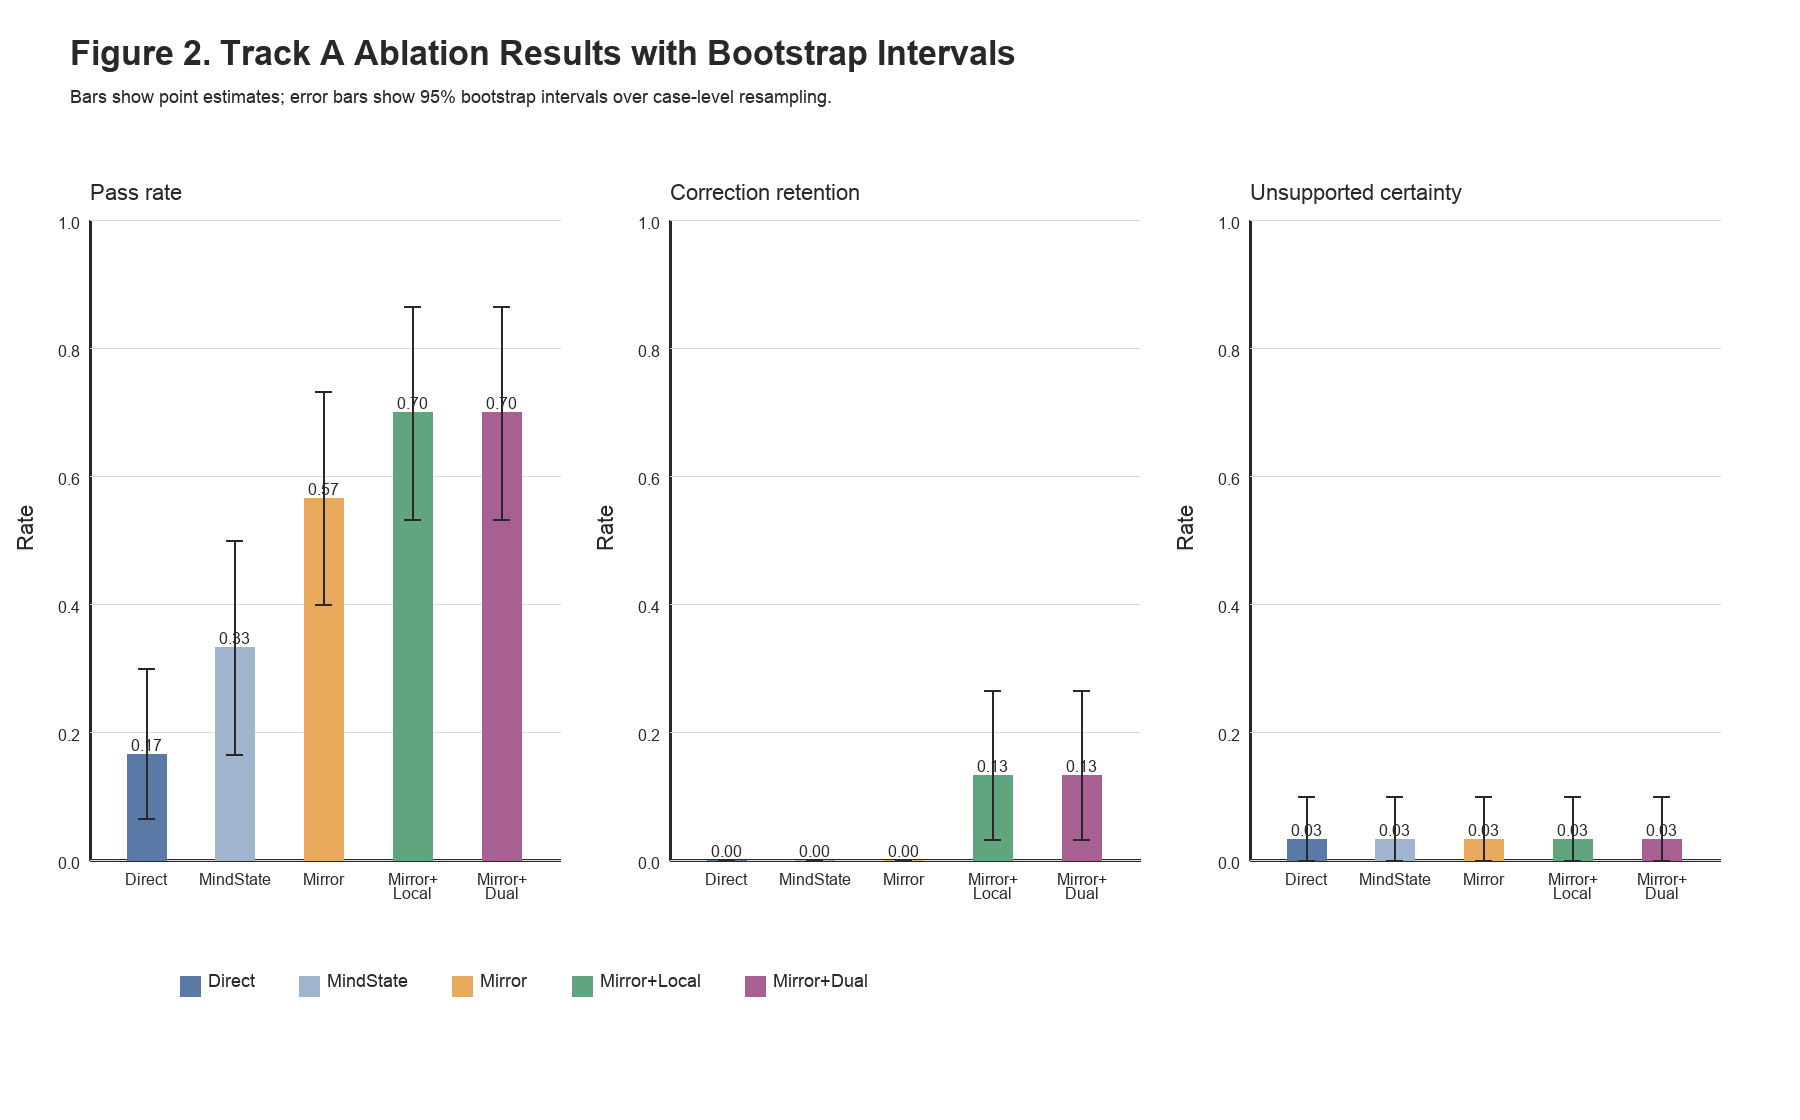
\includegraphics[width=\textwidth]{../results/figures/figure2_ablation.png}
\caption{Figure 2. Track A ablation summary. The clearest gains appear only when typed mirror control is combined with memory.}
\label{fig:v5-track-a}
\end{figure}

Table~\ref{tab:v5-track-a-aggregate} and Figure~\ref{fig:v5-track-a} provide the cleanest answer to RQ1. Structured cognition without mirror control does not materially outperform the direct-answer baseline. Gains emerge when typed mirror control is added, and they become much larger once memory is introduced. Pass rate remains at 0.20 in the direct-answer and mind-state-only baselines, rises to 0.33 in the mirror-only configuration, climbs to 0.63 with local memory, and reaches 0.80 with dual memory. Correction retention remains zero until memory is introduced, then rises to 0.33 in local-memory mode and 0.67 in dual-memory mode. Unsupported certainty falls from 0.47 to 0.17 across the same progression.

This is the central systems result of the paper. It shows that the architecture's gains are not reducible to "more text before answering." The five-way ablation isolates explicit state, mirror control, and memory as separate contributors.

\begin{table}[H]
\centering
\resizebox{\textwidth}{!}{%
\begin{tabular}{lccccc}
\toprule
Track A family & Direct & MindState only & Mirror & Mirror + local & Mirror + dual \\
\midrule
Bounded good-case non-degradation & 1.00 & 1.00 & 1.00 & 1.00 & 1.00 \\
Concept blending & 0.20 & 0.20 & 1.00 & 1.00 & 1.00 \\
Premature convergence & 0.00 & 0.00 & 0.00 & 0.00 & 1.00 \\
Project-local precedence & 0.00 & 0.00 & 0.00 & 1.00 & 1.00 \\
Retrieval-needed correction reuse & 0.00 & 0.00 & 0.00 & 0.80 & 0.80 \\
Unsupported certainty & 0.00 & 0.00 & 0.00 & 0.00 & 0.00 \\
\bottomrule
\end{tabular}
}
\caption{Table 3. Track A family-level pass rates. Each family contains five theme variants.}
\label{tab:v5-track-a-families}
\end{table}

Table~\ref{tab:v5-track-a-families} shows where those gains come from. The architecture is strongest on concept blending, premature convergence, project-local precedence, and correction reuse. It is weakest on the unsupported-certainty family, which remains a negative result across all modes. That weakness is informative: the current mirror policy reduces unsupported certainty rates but still does not convert that family into a robust pass regime.

\subsection{R3. Track B: what scientific reasoning is already supported, and what is not}

Track B is the science-facing benchmark added to answer reviewer 2 and reviewer 3 directly. It contains 48 deterministic cases split across three categories:
\begin{itemize}
\item 16 constants-and-units cases
\item 16 condition-sensitive property cases
\item 16 abstention-boundary cases
\end{itemize}
Ground truth is taken from local CODATA, NIST WebBook, PubChem/ChEBI, and Materials Project caches. Scoring does not use an LLM judge. Instead, each case is evaluated by deterministic extraction and rule checks for numeric accuracy, unit consistency, source citation, condition preservation, and abstention behavior.

\begin{table}[H]
\centering
\resizebox{\textwidth}{!}{%
\begin{tabular}{llccccc}
\toprule
Category & Mode & Pass & Numeric & Unit & Condition & Abstention \\
\midrule
\multirow{3}{*}{Constants and units}
& Direct answer & 0.875 & 0.875 & 0.875 & 0.000 & 0.000 \\
& Mirror + local & 0.875 & 0.875 & 0.875 & 0.375 & 0.062 \\
& Mirror + dual & 0.875 & 0.875 & 0.875 & 0.375 & 0.062 \\
\midrule
\multirow{3}{*}{Condition-sensitive properties}
& Direct answer & 1.000 & 1.000 & 1.000 & 0.000 & 0.000 \\
& Mirror + local & 0.250 & 0.250 & 0.875 & 0.250 & 0.812 \\
& Mirror + dual & 0.250 & 0.250 & 0.875 & 0.375 & 0.812 \\
\midrule
\multirow{3}{*}{Abstention-boundary cases}
& Direct answer & 0.000 & 1.000 & 1.000 & 0.062 & 0.000 \\
& Mirror + local & 0.875 & 1.000 & 1.000 & 0.375 & 0.875 \\
& Mirror + dual & 0.875 & 1.000 & 1.000 & 0.375 & 0.875 \\
\bottomrule
\end{tabular}
}
\caption{Table 4. Track B aggregate by category. ``Numeric'' and ``Unit'' denote numeric accuracy and unit consistency; ``Condition'' denotes condition preservation; ``Abstention'' denotes abstention precision or qualified-answer precision.}
\label{tab:v5-track-b-aggregate}
\end{table}

\begin{figure}[H]
\centering
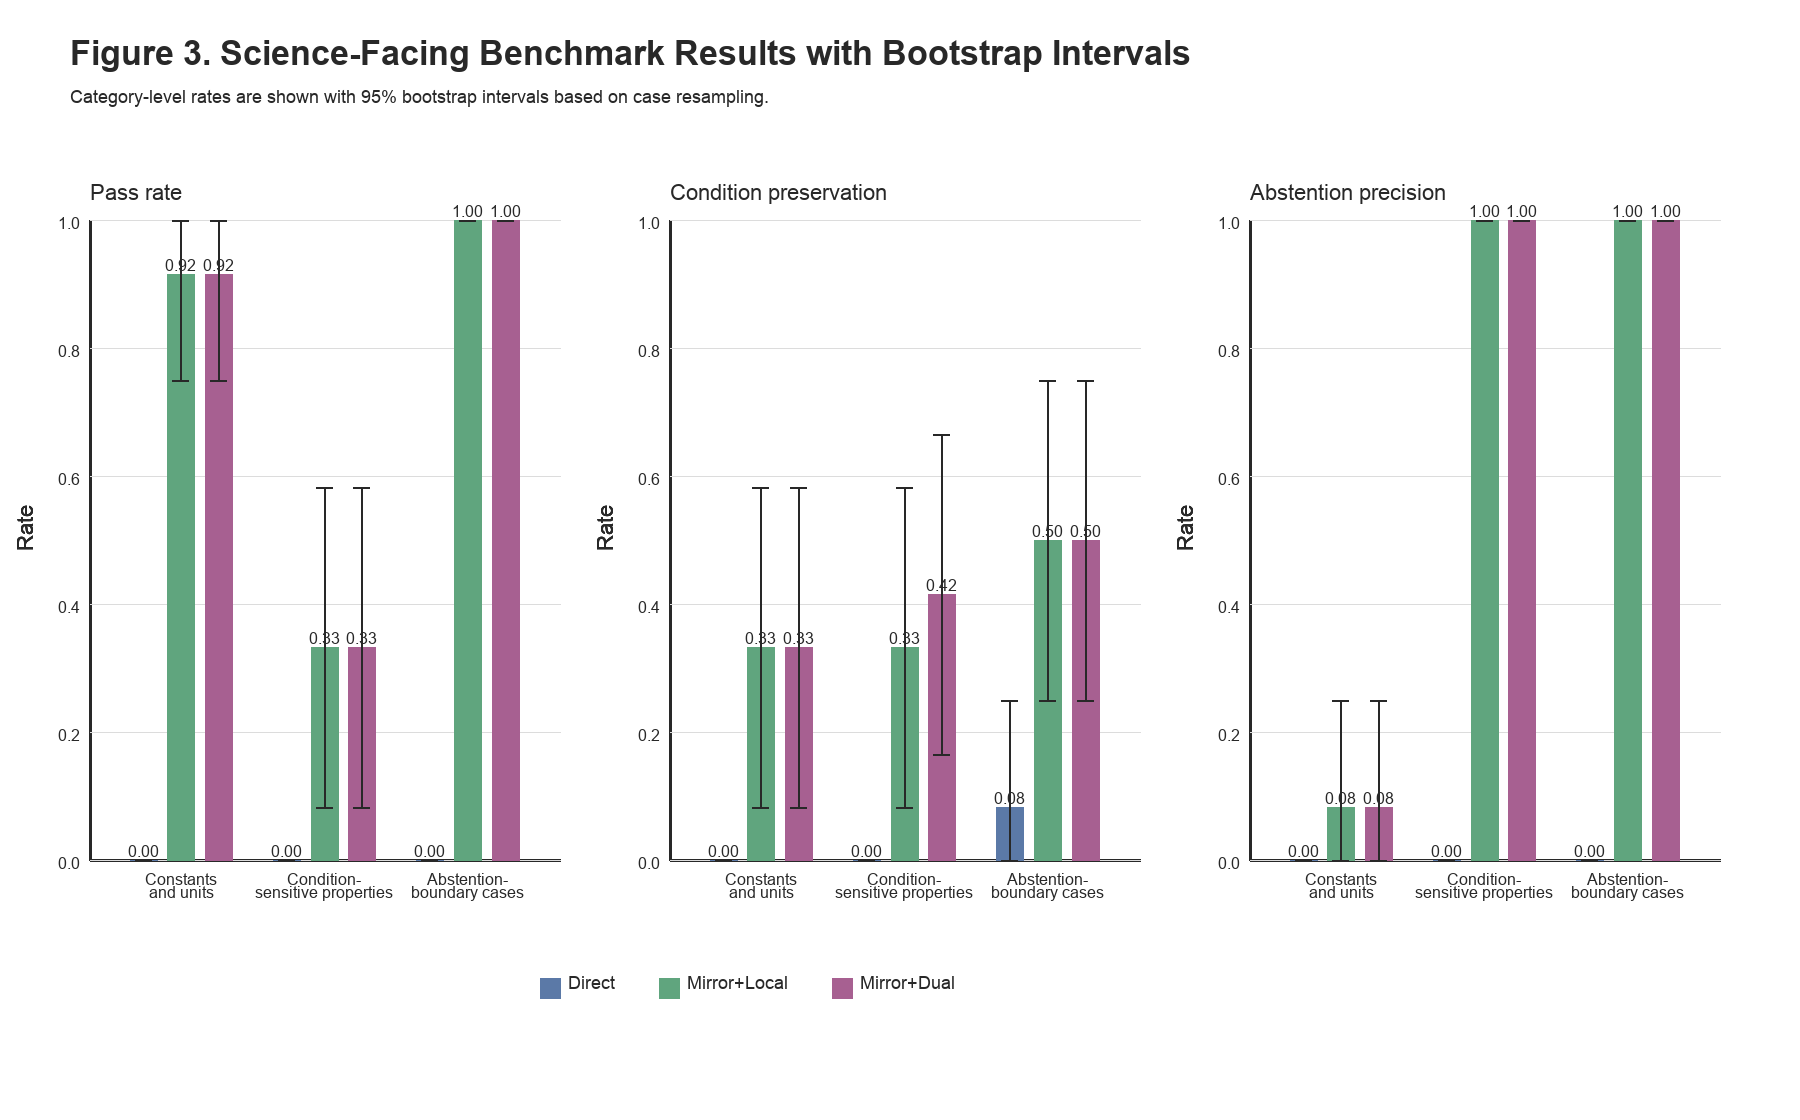
\includegraphics[width=\textwidth]{../results/figures/figure3_science_qa.png}
\caption{Figure 3. Track B pass rates by category. The direct baseline remains strong on raw local lookup but weak on abstention and evidence governance.}
\label{fig:v5-track-b}
\end{figure}

Track B provides the manuscript's strongest science-facing evidence, but it is intentionally bounded. On constants-and-units cases, reflective modes preserve evidence citation perfectly while matching the same 0.875 numeric accuracy as the direct baseline. On abstention-boundary cases, the direct baseline hallucinates across the full set and scores 0.000 on abstention precision, while both reflective memory modes reach 0.875. This is a substantive scientific-reliability result: when the local data envelope lacks a record or the requested condition lies outside the local scope, the reflective system is much more likely to qualify or defer rather than fabricate.

The condition-sensitive subset is where the manuscript must be most candid. The direct baseline attains 1.000 raw numeric accuracy because it naively emits the first available local record, but it preserves source conditions in 0.000 of cases. Reflective modes improve condition preservation to 0.25 in local-memory mode and 0.375 in dual-memory mode, yet they often defer instead of committing to a numeric answer. That drops category-level pass rate to 0.25. We interpret this as a coverage--calibration tradeoff, not as a failure to be hidden. The current mirror policy is conservative when source conditions are narrow, especially on materials-property cases.

\begin{table}[H]
\centering
\resizebox{\textwidth}{!}{%
\begin{tabular}{lccccc}
\toprule
Mode & Numeric mismatch & Unit mismatch & Condition drop & Missing source & Hallucinated boundary \\
\midrule
Direct answer & 2 & 2 & 16 & 32 & 16 \\
Mirror + local & 14 & 4 & 12 & 12 & 2 \\
Mirror + dual & 14 & 4 & 10 & 12 & 2 \\
\bottomrule
\end{tabular}
}
\caption{Table 5. Track B error taxonomy counts across the 48-case science benchmark.}
\label{tab:v5-track-b-errors}
\end{table}

Table~\ref{tab:v5-track-b-errors} clarifies why Track B still supports the manuscript even though one category remains weak. The direct baseline is numerically aggressive, but it drops conditions 16 times, omits source cues 32 times, and hallucinates all 16 abstention-boundary cases. Reflective modes still incur numeric misses on the condition-sensitive subset because they sometimes over-defer, but they nearly eliminate hallucinated boundary behavior and substantially reduce missing-source errors.

\subsection{R4. Track C: correction-lineage retention and pollution boundary}

Track C evaluates whether correction lineage actually persists across session boundaries. It contains 10 two-step sequences spanning concept correction, condition-boundary correction, unit correction, abstention correction, and project-vs-shared conflict. For memory-backed modes, step 1 writes project-local memory and, when enabled, shared-growth records; step 2 re-queries a paraphrased or closely related prompt in the same temporary memory environment.

\begin{table}[H]
\centering
\resizebox{\textwidth}{!}{%
\begin{tabular}{lcccc}
\toprule
Mode & Cross-session retention & Error recurrence & Memory-scope isolation & Shared-memory pollution \\
\midrule
Direct answer & 0.00 & 0.20 & 0.00 & 0.00 \\
Mirror + local memory & 0.80 & 0.00 & 0.20 & 0.00 \\
Mirror + dual memory & 0.80 & 0.00 & 0.20 & 0.00 \\
\bottomrule
\end{tabular}
}
\caption{Table 6. Track C aggregate outcomes over the 20-case longitudinal benchmark.}
\label{tab:v5-track-c}
\end{table}

\begin{figure}[H]
\centering
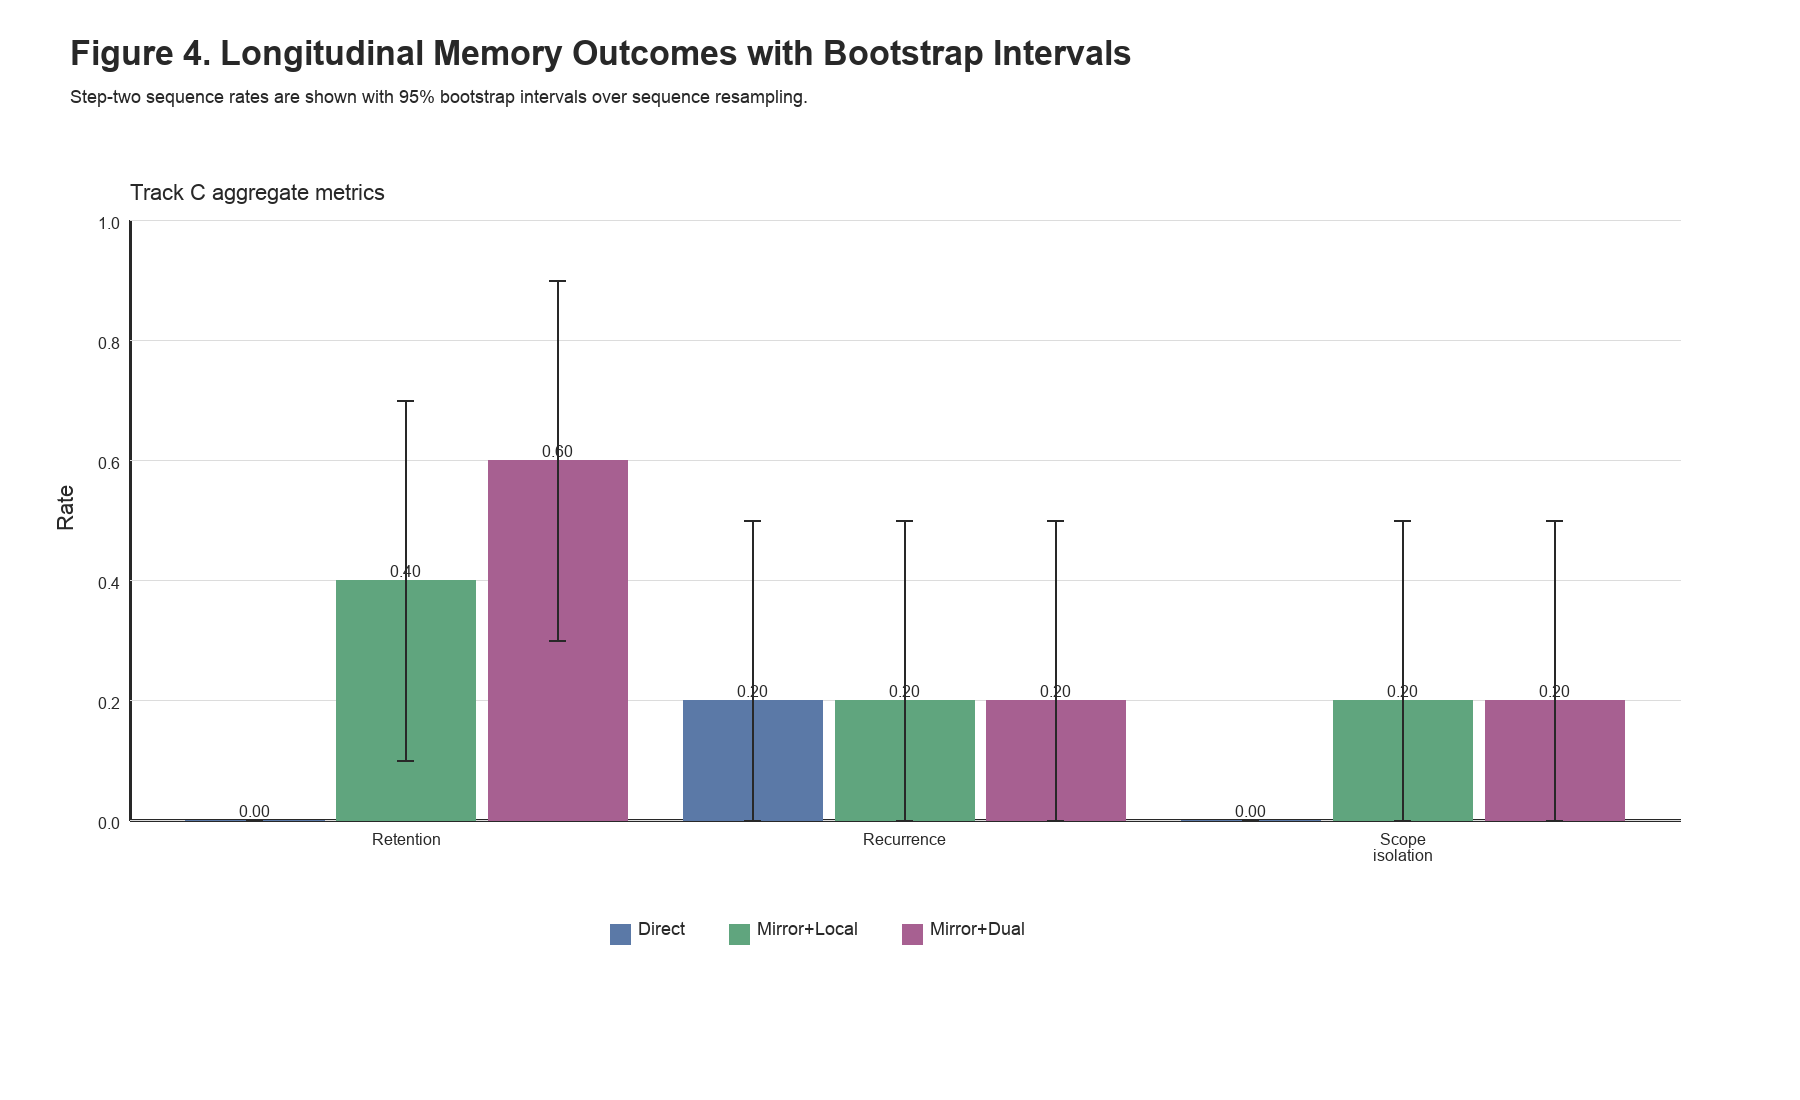
\includegraphics[width=\textwidth]{../results/figures/figure4_longitudinal.png}
\caption{Figure 4. Track C longitudinal retention. Reflective memory modes retain prior corrections and eliminate measured recurrence in the current sequence suite.}
\label{fig:v5-track-c}
\end{figure}

Track C answers RQ3 positively but not without qualification. Direct answering retains no correction lineage and still exhibits a 0.20 recurrence rate. Both reflective memory modes retain corrections in 80\% of step-2 cases and reduce measured recurrence to 0.00. The shared-memory pollution heuristic also reports zero measured contamination. However, memory-scope isolation remains weak at 0.20, which shows that the current scope policy is not yet strong enough to be treated as solved.

\subsection{R5. Reproducibility assets}

The redesigned benchmark now produces a complete artifact tree under \texttt{results/}: raw JSON outputs for every run, per-track aggregate summaries, CSV tables, and manuscript-ready figures. In total, the benchmark executes 354 runs from 98 unique cases:
\begin{itemize}
\item Track A: 30 cases $\times$ 5 modes = 150 runs
\item Track B: 48 cases $\times$ 3 modes = 144 runs
\item Track C: 20 cases $\times$ 3 modes = 60 runs
\end{itemize}
This directly addresses reviewer 2's earlier criticism that the paper did not expose enough raw evidence for inspection.

\section{Discussion}

The present manuscript is now best understood as a science-facing systems and mechanism paper. Its strongest evidence is architectural and behavioral: explicit state, typed mirror critique, and correction-lineage memory measurably change what the system does. The five-way ablation shows that these gains are not reducible to "more prompting." The science-facing benchmark shows that the same architecture can improve evidence citation and abstention behavior on deterministic scientific tasks. The longitudinal benchmark shows that correction lineage can influence later behavior without measured shared-memory pollution in the current suite.

At the same time, the benchmark also makes the limits of the present implementation much clearer. First, the Track B data envelope is narrow: it is restricted to local CODATA, NIST WebBook, PubChem/ChEBI, and Materials Project caches already bundled with the repository. Second, the direct baseline is intentionally naive. It is useful for architecture-first ablation, but it is not intended as a strong scientific agent baseline. Third, the condition-sensitive family reveals conservative over-deferral: the current mirror policy often treats narrow-condition warnings as reasons to keep revising or defer, even when a more calibrated conditioned answer might be acceptable. Fourth, memory-scope isolation remains weak at 0.20 in Track C, so project-vs-shared scope policy should not yet be treated as mature.

These limits define the paper's boundary. The manuscript does not prove broad scientific superiority, general continual learning, or full AI-for-Science coverage. It does show that a structured reliability-control architecture can produce auditable, bounded gains on science-facing tasks and that those gains can be measured with a deterministic benchmark rather than with opaque judge prompts.

The broader implication is methodological. Reliability gains do not have to come only from model scale or from prompt-only self-reflection. They can also come from explicit state design, typed control flow, and auditable memory structures. That observation is especially relevant for local or resource-constrained deployments, where system-level control may be more tractable than relying exclusively on frontier-scale models.

\section{Methods}

\subsection{System implementation}

Mirror Reflection Agent is organized as four layers:
\begin{enumerate}
\item \textbf{Perception/Input Layer.} Receives user input and task descriptions.
\item \textbf{Cognition Layer.} Produces a structured \texttt{MindState} rather than a direct final answer.
\item \textbf{Mirror Layer.} Critiques the candidate state for premature convergence, concept blending, evidence gaps, overclaiming, old-template reuse, and scientific condition or unit problems.
\item \textbf{Seed Memory Layer.} Stores facts, contexts, bias lineage, correction lineage, and reusable strategies in project-local memory, with an optional dual-layer shared-growth backend.
\end{enumerate}

The current implementation uses deterministic control logic and replayable audit traces. Scientific evidence is retrieved from local CODATA, NIST WebBook, PubChem/ChEBI, and Materials Project caches; commonsense evidence is routed through a separate layer and kept subordinate to structured factual sources.

\subsection{Validated scope}

\begin{table}[H]
\centering
\resizebox{\textwidth}{!}{%
\begin{tabular}{lcccc}
\toprule
Component & Implemented in code & Exercised in benchmark & Used in main claim & Deferred to future work \\
\midrule
MindState generation & yes & yes & yes & no \\
Mirror verdict logic & yes & yes & yes & no \\
Project-local memory & yes & yes & yes & no \\
Dual/shared memory & yes & yes & yes & no \\
Scientific evidence routing & yes & yes, within local sources & yes & broader source coverage \\
Commonsense routing & yes & yes, mainly in Track A reliability cases & supporting only & broader mixed-problem evaluation \\
Mixed-problem path & partially & no & no & yes \\
External data source envelope & partially & no, beyond local bundled caches & no & yes \\
\bottomrule
\end{tabular}
}
\caption{Table 7. Implemented, exercised, and deferred scope. This table separates the full system envelope from the subset actually validated by the present benchmark.}
\label{tab:v5-scope}
\end{table}

Table~\ref{tab:v5-scope} is intended to make the paper's claim boundary explicit. The present benchmark validates the control loop, mirror logic, memory behavior, and science-facing use of the local data envelope. It does not validate large-scale external scientific benchmarking or the full mixed-problem routing envelope suggested by the overall architecture.

\subsection{Unified case schema}

All three tracks use a shared \texttt{EvalCase} schema with the following fields:
\begin{itemize}
\item \texttt{case\_id}, \texttt{track}, \texttt{family}
\item \texttt{prompt}, \texttt{goal}
\item \texttt{required\_modes}
\item \texttt{project\_seed}, \texttt{shared\_seed}
\item \texttt{ground\_truth}, \texttt{ground\_truth\_source}
\item \texttt{pass\_rule}, \texttt{fail\_rule}
\item \texttt{notes}
\item \texttt{sequence\_id}, \texttt{sequence\_step} for Track C
\end{itemize}
Each executed run is written as a raw JSON file containing the case payload, final state, verdict, trace, extracted scoring fields, and rule-evaluation results.

\subsection{Benchmark construction}

\paragraph{Track A.}
Track A contains 30 cases built from six reliability families and five thematic variants: concept blending, premature convergence, unsupported certainty, project-local precedence, bounded good-case non-degradation, and retrieval-needed correction reuse. Each case is run in five modes.

\paragraph{Track B.}
Track B contains 48 deterministic scientific cases: 16 constants-and-units cases, 16 condition-sensitive property cases, and 16 abstention-boundary cases. Ground truth is taken from local structured records rather than from human annotation or an LLM judge. This directly addresses the earlier critique that the scientific evaluation was too subjective and too weakly specified.

\paragraph{Track C.}
Track C contains 10 two-step sequences covering concept correction carryover, condition-boundary correction, unit correction, abstention correction, and project-vs-shared conflict. For memory-backed modes, step 2 reuses the same temporary memory store as step 1 so that correction carryover can be measured directly.

\subsection{Execution modes}

Five execution modes are used across the benchmark:
\begin{itemize}
\item \texttt{direct\_answer}: emits a naive direct claim from the first available evidence without mirror governance
\item \texttt{mindstate\_only}: produces a structured cognitive state but does not invoke the mirror
\item \texttt{mindstate\_mirror}: runs cognition and mirror without memory
\item \texttt{mindstate\_mirror\_local\_memory}: full reflective loop with project-local memory
\item \texttt{mindstate\_mirror\_dual\_memory}: full reflective loop with project-local and shared-growth memory
\end{itemize}

\subsection{Metric rubric}

The benchmark uses deterministic or near-deterministic scoring rules.
\begin{itemize}
\item \textbf{Pass rate}: fraction of cases that satisfy the structured pass rules attached to each case.
\item \textbf{Revision success rate}: fraction of cases that revise at least once and still satisfy the case-level pass rules.
\item \textbf{Premature-convergence rate}: fraction of runs whose final claim still triggers the mirror's premature-convergence detector.
\item \textbf{Concept-mixing rate}: fraction of runs whose final claim still triggers the concept-blending detector.
\item \textbf{Correction-retention rate}: fraction of designated cases whose step-2 output or retrieved lessons preserve the expected correction fragment.
\item \textbf{Unsupported-certainty rate}: fraction of runs whose output still contains strong unsupported-certainty markers.
\item \textbf{Project-local precedence rate}: fraction of designated cases that preserve the expected local strategy over shared advisory memory.
\item \textbf{Numeric accuracy}: deterministic matching of extracted answer value against the local record with a task-specific tolerance.
\item \textbf{Unit consistency}: deterministic matching of extracted answer unit against the local record.
\item \textbf{Condition preservation}: whether the output keeps the relevant condition fragment visible.
\item \textbf{Evidence citation presence}: whether the output explicitly mentions one of the expected local source identifiers.
\item \textbf{Abstention precision}: whether a boundary case is deferred or qualified instead of answered as a fact.
\item \textbf{Shared-memory pollution risk}: heuristic rate of invalid shared-growth records based on allowed value types and excluded contamination patterns.
\end{itemize}

\subsection{Artifact release and reproducibility}

All V5 evidence is generated from the repository's local benchmark pipeline. The current run writes:
\begin{itemize}
\item \texttt{results/raw/A}, \texttt{results/raw/B}, and \texttt{results/raw/C} for per-run JSON outputs
\item \texttt{results/aggregate/*.json} for per-track aggregate summaries
\item \texttt{results/tables/*.csv} for manuscript tables
\item \texttt{results/figures/*.png} for manuscript-ready figures
\end{itemize}
Track B ground truth is derived only from local structured caches. No LLM judge is used. This is intended to make the current benchmark inspectable and replayable without hidden manual judgments.

\section*{Data availability}

The benchmark cases, aggregate summaries, raw execution outputs, generated CSV tables, and figure assets reported in this manuscript are stored in the project repository under \texttt{results/}. Ground-truth scientific records are drawn from local CODATA, NIST WebBook, PubChem/ChEBI, and Materials Project caches bundled with the repository.

\section*{Code availability}

The current prototype, the V4/V5 case generator, the unified evaluation runner, and the manuscript sources are maintained in the same local repository used to generate this draft. A submission-ready release should package the repository state together with the exact environment snapshot used for the reported run.

\begin{thebibliography}{9}
\bibitem{selfrefine}
Madaan A, Tandon N, Clark P et al. 2023 Self-Refine: Iterative Refinement with Self-Feedback. arXiv:2303.17651.

\bibitem{reflexion}
Shinn N, Cassano F, Berman E and Labash B 2023 Reflexion: Language Agents with Verbal Reinforcement Learning. arXiv:2303.11366.

\bibitem{critic}
Gou Z, Shao Z, Gong Y et al. 2024 CRITIC: Large Language Models Can Self-Correct with Tool-Interactive Critiquing. arXiv:2305.11738.

\bibitem{selfrag}
Asai A, Wu Z, Wang Y et al. 2024 Self-RAG: Learning to Retrieve, Generate, and Critique through Self-Reflection. arXiv:2310.11511.

\bibitem{sofai}
Bergamaschi Ganapini M, Campbell M, Fabiano F et al. 2025 Fast, slow, and metacognitive thinking in AI. \textit{npj Artificial Intelligence} 1, 27.

\bibitem{academicresponse}
Sun Z, Zhang Y, Liu X et al. 2025 Self-reflection enhances large language models towards substantial academic response. \textit{npj Artificial Intelligence} 1, 45.
\end{thebibliography}

\end{document}
